\documentclass[main.tex,fontsize=6pt,paper=a4,paper=landscape,DIV=calc,]{scrartcl}
% Document
\usepackage[T1]{fontenc}
\usepackage[utf8]{inputenc}
\usepackage[dvipsnames]{xcolor}
\usepackage[nswissgerman,english]{babel} 
\usepackage{hyperref}
\renewcommand{\familydefault}{\sfdefault}

% Format
\usepackage[top=5mm,bottom=5mm,left=5mm,right=5mm]{geometry}
%\setlength{\headheight}{\baselineskip}
%\setlength{\headsep}{0mm}

%\usepackage{scrlayer-scrpage}
%\clearpairofpagestyles
%\chead{{\bfseries\TITLE, \AUTHOR, \pagename~\thepage}}

%\addtokomafont{pagehead}{\upshape}

\usepackage{multicol}
\setlength{\columnsep}{2mm}
\setlength{\columnseprule}{0.1pt}

% Math
\usepackage{amsmath}
\usepackage{amssymb}
\usepackage{amsfonts}

% Code
\usepackage{fancyvrb, etoolbox, listings, xcolor}
%\usemintedstyle{bw}

%\newminted[shell]{bash}{
%fontsize=\footnotesize,
%fontfamily=tt,
%breaklines=true,
%frame=single,
%framerule=0.1pt,
%framesep=2mm,
%tabsize=2
%}
%\newminted{css}{
%breaklines=true,
%tabsize=4,
%autogobble=true,
%escapeinside=||,
%stripall=true,
%stripnl=true,
%}

    \definecolor{lightgray}{rgb}{0.95, 0.95, 0.95}
    \definecolor{darkgray}{rgb}{0.4, 0.4, 0.4}
    \definecolor{purple}{rgb}{0.65, 0.12, 0.82}
    \definecolor{ocherCode}{rgb}{1, 0.5, 0} % #FF7F00 -> rgb(239, 169, 0)
    \definecolor{blueCode}{rgb}{0, 0, 0.93} % #0000EE -> rgb(0, 0, 238)
    \definecolor{greenCode}{rgb}{0, 0.6, 0} % #009900 -> rgb(0, 153, 0)
    \definecolor{teal}{rgb}{0.0, 0.5, 0.5}

\lstdefinestyle{code}{
    identifierstyle=\color{black},
    keywordstyle=\color{blue}\bfseries\small,
    ndkeywordstyle=\color{greenCode}\bfseries\small,
    stringstyle=\color{ocherCode}\ttfamily\small,
    commentstyle=\color{teal}\ttfamily\textit\small,
    basicstyle=\ttfamily\small,
    breakatwhitespace=false,         
    breaklines=true,                 
    captionpos=b,                    
    keepspaces=true,                 
    showspaces=false,                
    showstringspaces=false,
    showtabs=false,                  
    tabsize=2,
    belowskip=-5pt
}



% Images
\usepackage{graphicx}
\newcommand{\pic}{\includegraphics[scale=0.3]}
\graphicspath{{Screenshots/}{../Screenshots}}
\makeatletter
\def\pictext#1#2{%
    \@ifnextchar[{%
    \pictext@iiiii{#1}{#2}%
    }{%
      \pictext@iiiii{#1}{#2}[0.5,0.4,0.3]% Default is 5
    }%
}
\def\pictext@iiiii#1#2[#3,#4,#5]{\begin{minipage}{#3\textwidth}\includegraphics[scale=#4]{#1}\end{minipage}\begin{minipage}{#5\textwidth}#2\end{minipage}}
\def\minipg#1#2{%
    \@ifnextchar[{%
    \minipg@iiii{#1}{#2}%
    }{%
      \minipg@iiii{#1}{#2}[0.3,0.6]% Default is 5
    }%
}
\def\minipg@iiii#1#2[#3,#4]{\vspace{0.8mm}\begin{minipage}{#3\textwidth}#1\end{minipage}\begin{minipage}{#4\textwidth}#2\end{minipage}{\vspace{0.8mm}}}
\makeatother

%\newenvironment{minty}[2]% environment name
%{% begin code
%  \begin{minipage}{#1}
%  \begin{minted}{#2}
%}%
%{% end code
%  \end{minted}
%  \end{minipage}
%  \end{minty}\ignorespacesafterend
%} 

% Smaller Lists
\usepackage{enumitem}
\setlist[itemize,enumerate]{leftmargin=3mm, labelindent=0mm, labelwidth=1mm, labelsep=1mm, nosep}
\setlist[description]{leftmargin=0mm, nosep}
\setlength{\parindent}{0cm}

% Smaller Titles
\usepackage[explicit]{titlesec}

%% Color Boxes
\newcommand{\sectioncolor}[1]{\colorbox{black!60}{\parbox{0.97\linewidth}{\color{white}#1}}}
\newcommand{\subsectioncolor}[1]{\colorbox{black!50}{\parbox{0.97\linewidth}{\color{white}#1}}}
\newcommand{\subsubsectioncolor}[1]{\colorbox{black!40}{\parbox{0.97\linewidth}{\color{white}#1}}}
\newcommand{\paragraphcolor}[1]{\colorbox{black!30}{\parbox{0.97\linewidth}{\color{white}#1}}}
\newcommand{\subparagraphcolor}[1]{\colorbox{black!20}{\parbox{0.97\linewidth}{\color{white}#1}}}

%% Title Format
\titleformat{\section}{\vspace{0.3mm}\bfseries}{}{0mm}{\sectioncolor{\thesection~#1}}[{\vspace{0.3mm}}]
\titleformat{\subsection}{\vspace{0.3mm}\bfseries}{}{0mm}{\subsectioncolor{\thesubsection~#1}}[{\vspace{0.3mm}}]
\titleformat{\subsubsection}{\vspace{0.3mm}\bfseries}{}{0mm}{\subsubsectioncolor{\thesubsubsection~#1}}[{\vspace{0.3mm}}]
\titleformat{\paragraph}{\vspace{0.3mm}\bfseries}{}{0mm}{\paragraphcolor{\theparagraph~#1}}[{\vspace{0.3mm}}]
\titleformat{\subparagraph}{\vspace{0.3mm}\bfseries}{}{0mm}{\subparagraphcolor{\thesubparagraph~#1}}[{\vspace{0.3mm}}]

%% Title Spacing
\titlespacing{\section}{0mm}{0mm}{0mm}
\titlespacing{\subsection}{0mm}{0mm}{0mm}
\titlespacing{\subsubsection}{0mm}{0mm}{0mm}
\titlespacing{\paragraph}{0mm}{0mm}{0mm}
\titlespacing{\subparagraph}{0mm}{0mm}{0mm}

%% format cells
\usepackage[document]{ragged2e}
\usepackage{array, makecell}
\renewcommand{\arraystretch}{2}
\newcommand{\mc}{\makecell[{{m{1\linewidth}}}]}



\lstdefinelanguage{JavaScript}{
  keywords={break, case, catch, continue, debugger, default, delete, do, else, false, finally, for, function, if, in, instanceof, new, null, return, switch, this, throw, true, try, typeof, var, void, while, with},
  morecomment=[l]{//},
  morecomment=[s]{/*}{*/},
  morestring=[b]',
  morestring=[b]",
  ndkeywords={class, export, boolean, throw, implements, import, this},
  keywordstyle=\color{blue}\bfseries,
  ndkeywordstyle=\color{darkgray}\bfseries,
  identifierstyle=\color{black},
  commentstyle=\color{purple}\ttfamily,
  stringstyle=\color{red}\ttfamily,
  sensitive=true
}

%%%%%define html as viable language
\lstset{
    language=JavaScript,
    style=code,
}
%%%%%

\newcommand{\TITLE}{Web Engineering 1}
\newcommand{\AUTHOR}{Fabio Lenherr / Felix Tran}
\setcounter{tocdepth}{1}

\begin{document}
\begin{multicols*}{4}
% \tableofcontents

\section{Basics}

\subsection{ECMAScript} 
Javascript is only an implementation of ECMAScript. So ECMA is the actual standard.
 
\subsection{Primitives vs Objects}  
\textcolor{red}{Primitives}

\begin{itemize}
  \item \textcolor{teal}{string, number, boolean, undefined}
  \item \textcolor{teal}{compared by value}
  \item \textcolor{teal}{immutable: you can't change a number, only a variable!}
\end{itemize}
\vspace{2mm}
\textcolor{red}{Objects}
\begin{itemize}
  \item \textcolor{teal}{Arrays, Regular Expressions, Functions}
  \item \textcolor{teal}{compared by Reference}
  \item \textcolor{teal}{Mutable by default}
\end{itemize}


\subsection{Types} 
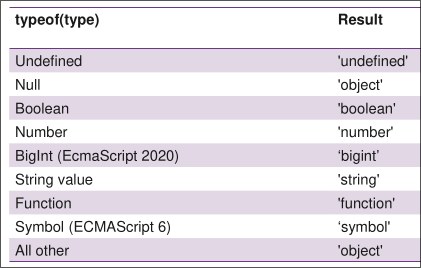
\includegraphics[width=0.8\columnwidth]{2022-10-11-10_33_44.png}

\subsection{Automatic casting to Integer}
\textcolor{purple}{Engines try to represent floats as integers if possible:}
\vspace{-2mm}
\begin{lstlisting}
console.log(0.3333333333333333 * 3 == 1);  //true
let x = 1/3;                               
console.log(x + x + x);                    //1
console.log(0.3 + 0.7);                    //1
console.log(Number.isInteger(x + x + x));  //true
console.log(Number.isInteger(0.3));        //false
console.log(0.1 + 0.2);       //0.3000000000000004

// however sometimes it is out of bounds:
console.log(99999999999999999); //100000000000000000
Number.isSafeInteger(99999999999999999); //false
\end{lstlisting}
\vspace{2mm}

\subsection{Boolean Checks}  
\textcolor{red}{Every value can be converted to a boolean}\newline
\begin{itemize}
  \item !!(null) => false
  \item Boolean( null ) => false
\end{itemize}
\begin{itemize}
  \item \textcolor{teal}{Logical Operators || \&\&}
  \item \textcolor{teal}{Not !}
  \item \textcolor{teal}{Equality Checks === !== > >= < <=} true or false
  \item \textcolor{teal}{Value Equality Check == !=} true false or NaN(cast to number)
\end{itemize}
\minipg{
False Values:
\begin{itemize}
  \item false
  \item 0 
  \item "" 
  \item null 
  \item undefined 
  \item NaN
  \, \newline
\end{itemize}
}{
True Values:
\begin{itemize}
  \item "0" 
  \item "false"
  \item \char`\[ \char`\]
  \item \char`\{ \char`\}
\end{itemize}
\textcolor{teal}{any string that has something in it is considered true}
}[0.1,0.1]
 
\subsection{NaN} 
\begin{itemize}
  \item \textcolor{red}{is an error value} 
  \item 0 / 0 = NaN
  \item is of type number
  \item NaN == NaN is false \textcolor{teal}{// use isNan\char`\( \char`\) instead}
  \item NaN === NaN is false 
\end{itemize}

\subsection{Infinity}  
Infinity is a number in js, can be used to represent the mathematical infinity.\newline
Will also be used if the number is too big!

\subsection{Numbers}  
\textcolor{red}{Every value can be casted to a number!}\newline
\begin{itemize}
  \item +(true) = 1
  \item Number(true) = 1
  \item Number(null) = 0
  \item Number("abc") = NaN \textcolor{teal}{remember NaN is of type number!}
  \item one exception -> symbol, this is not a number\newline
    Error would be: Uncaught TypeError: Cannot convert a Symbol value to a number
  \item You can explicitly convert string to number with \emph{parseInt() and parseFloat()} 
\end{itemize}

\subsection{String}  
\textcolor{teal}{Can be represented with either "" or ''}\newline
\textcolor{teal}{Escape character is \textbackslash}\newline
\minipg{
Typical Methods:
\begin{itemize}
  \item length
  \item slice
  \item trim\char`\( \char`\)
  \item includes\char`\( \char`\)
  \item indexOf\char`\( \char`\)
\end{itemize}
}
{
  Special Operations:
  \begin{itemize}
  \item \textcolor{red}{Number + String = String}
  \item \textcolor{red}{String + Number = String}
  \, \newline
  \, \newline
  \, \newline
  \end{itemize} 
}[0.1, 0.15]
\vspace{-2mm}
\begin{lstlisting}
`Composition string ${var}` // string with variables
\end{lstlisting}
\vspace{2mm}

\subsection{null / undefined}  
\textcolor{teal}{Undefined means nothing, not yet defined}\newline
\textcolor{teal}{null is a value, the null value}\newline
\textcolor{red}{IMPORTANT: null == undefined = true !!\newline While: null === undefined = false}\newline
Example with null and undefined:
\vspace{-2mm}
\begin{lstlisting}
console.log(a); // undefined -> a not defined
let a; // a still undefined as not initialized!
// null is either set specifically, or happens when a function should return a value but doesn't
\end{lstlisting}
\vspace{2mm}
Note that functions like console.log return undefined -> void.


\subsection{Array}  
\vspace{-2mm}
\begin{lstlisting}
const arr = [ 'a', 'b', 'c' ];
arr[0] = 'x';
arr.push("d");
console.log(arr); // [ 'x', 'b', 'c', 'd' ]
console.log(arr.length); // 4
\end{lstlisting}
\vspace{2mm}
This is the list for everything.\newline
\begin{itemize}
  \item \textcolor{teal}{no fix length}
  \item \textcolor{teal}{index starts at 0}
  
\end{itemize}
\textcolor{orange}{\textbf{To check if something is an array you can compare constructors!}}\newline
\vspace{-2mm}
\begin{lstlisting}
function isArray(arr) {
  if(arr.constructor === Array) {
    return true;
  }
  return false;
}
\end{lstlisting}
\vspace{2mm}
\textcolor{teal}{arr.forEach}\newline
\vspace{-2mm}
\begin{lstlisting}
let sum = 0;
arr.forEach(num => { sum += num });
\end{lstlisting}
\vspace{2mm}
\textcolor{teal}{Other array functions}\newline
\vspace{-2mm}
\begin{lstlisting}
const sum = arr.reduce((total, n) => total + n, 0); 
// sum of all elements in array, last value is 0(2nd param)
const mapped = arr.map((x) => x * 2); // all values doubled
const some = arr.some((x) => x === 0); 
// true if one value in the array has value 0
const every = arr.every((x) => x === 0); 
// true if all values are 0
const filter = arr.filter((x) => x === 0); 
// filter is a new array with all NON 0 values removed
const sort = arr.sort((a,b) => { return a - b});
// note the a - b -> in js needs to return number!! not bool!
\end{lstlisting}
\vspace{2mm}
\textcolor{purple}{Note that you can omit brackets when using only 1 param, or 1 line. If you use {} specifically, remember to write \emph{return}!!}


\subsection{For Loops}  
\textcolor{teal}{classic:}
\vspace{-2mm}
\begin{lstlisting}
for(let i=0; i<arr.length; ++i) {
  console.log("for",arr[i]);
} // like regular loop just with let
\end{lstlisting}
\vspace{2mm}
\textcolor{teal}{For-In:}
\vspace{-2mm}
\begin{lstlisting}
for(const x in arr) {
  console.log("for in", x + ":" + arr[x]);
} // !! this returns the index string not the element !!
\end{lstlisting}
\vspace{2mm}
\textcolor{teal}{For-Of:}
\vspace{-2mm}
\begin{lstlisting}
for(const y of arr) {
  console.log("for of", y);
} // like for(auto e : arr)
\end{lstlisting}
\vspace{2mm}


\subsection{Object}  
\textcolor{teal}{An object is a collection of properties}\newline
These values are stored in a \textbf{key | value} -> \textbf{HashSet}.
\vspace{-2mm}
\begin{lstlisting}
cosnt person = {
  name: "spass"
  func: function() {
    return this.name;
  }
};
person.name = "Bob";
person.os = "penguin"; // you can add properties on the fly!
person.func = function() { // or override functions!
  console.log("this does something else now !");
}
\end{lstlisting}
\vspace{2mm}

\subsection{Const}
\textcolor{purple}{In JS, just because the object is const, doesn't mean the underlying data of it is!}
\vspace{-2mm}
\begin{lstlisting}
const player = {
    name: '',
    id: 0,
};
player.id = 5; // works!!!
player = otherplayer; // ERROR
\end{lstlisting}
\vspace{2mm}

\subsection{Functions} 
\textcolor{teal}{As expected, functions are first class citizens, aka they can be variables!}
\vspace{-2mm}
\begin{lstlisting}
func = printSomething() {
  console.log("ping pang");
}
func();
\end{lstlisting}
\vspace{2mm}
Or You can use something like lambdas:
\vspace{-2mm}
\begin{lstlisting}
const func = (value) => {
  console.log(value);
}
func(5); // prints 5
\end{lstlisting}
\vspace{2mm}

\subsection{Parameters}  
\textcolor{red}{in javascript you can call functions with too many parameters, they will simply be stored in a buffer!!}
\vspace{-2mm}
\begin{lstlisting}
function foo(name, ...params){
console.log(1,name);
console.log(2,params.join(";"));
}
foo("Michael", "Gfeller", "OST", "IFS");
// prints "Michael" and "Gfeller;OST;IFS"
\end{lstlisting}
\vspace{2mm}

  \textcolor{teal}{Properties of functions}
\vspace{-2mm}
\begin{lstlisting}
const fn1 = function(){ return "Michael" };
console.log(fn1.name);
// "" -> function is anonymous
const fn2 = function name(){ return "Michael" };
console.log(fn2.name);
// "name" -> this is the name of the function

console.log(fn2.length); // 0 -> function has 0 params
const fn3 = function name(name){ return name };
console.log(fn3.length); // 1 -> function has 1 param
\end{lstlisting}
\vspace{2mm}

\subsubsection{Default Parameters}
\vspace{-2mm}
\begin{lstlisting}
function something(name = "henlo") {
  console.log(name);
}
something(); // henlo
something("birb"); // birb
\end{lstlisting}
\vspace{2mm}

\subsection{Overloading}
 \textcolor{red}{!!! Javascript doesn't have function overloading !!!}\newline
 The solution is to use if statements inside those functions with \textbf{typeof}
\vspace{-2mm}
\begin{lstlisting}
jQuery.fn.init = function( selector, context ) {
  if ( !selector ) {
  return this;
  }
  // Handle HTML strings
  if ( typeof selector === "string" ) {
    //...
  } else if ( jQuery.isFunction( selector ) ) {
    //...
  }
return jQuery.makeArray( selector, this );
};
\end{lstlisting}
\vspace{2mm}

\section{DOM Document Object Model}

\subsection{window}  
This simply provides global objects such as \textbf{console, document and HTMLDocument}\newline
\textcolor{teal}{All global variables reside here.}

Selection 
\textcolor{orange}{There are different ways of selecting an element or node:}
\begin{itemize}
  \item \textcolor{teal}{document.querySelector('name')} // select by CSS syntax -> also allows css selectors!
  \item \textcolor{teal}{document.querySelectorAll('.nav')} // select All by CSS syntax -> also allows css selectors!
  \item \textcolor{teal}{document.getElementById('list-container')} // select by id
  \item \textcolor{teal}{document.getElementByTagName('li')} // select by Tag name
  \item \textcolor{teal}{document.getElementsByClassName('nav-item')} // select by class name
\end{itemize}
Just use the querySelector -> it allows more ways to select it! \newline
However theoretically the html selectors are faster!

\subsection{DOM-Manipulation by create}  
\textcolor{orange}{We can also create new elements with js the same way we select elements}
\vspace{-2mm}
\begin{lstlisting}
const newEl = document.createElement('div');
newEl.appendChild(document.createTextNode('Hello'));
document.querySelector("#container").appendChild(newEl);
\end{lstlisting}
\vspace{2mm}
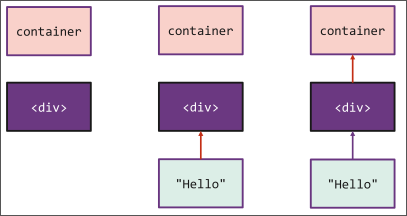
\includegraphics[width=0.7\columnwidth]{2022-10-18-11_26_10.png}\newline 
\textcolor{purple}{this is faster with small changes, DOM references stay the same, event handlers stay alive}

\subsection{DOM-Manipulation by innerHTML}  
\vspace{-2mm}
\begin{lstlisting}
const c = document.querySelector('#container');
c.innerHTML = '<div>Ping pang!</div>';
\end{lstlisting}
\vspace{2mm}
\textcolor{orange}{this is likely faster and more readable}
 
\subsection{DocumentFragment}  
This creates a temporary fragment that will be deleted when attaching this to a parent node.
\vspace{-2mm}
\begin{lstlisting}
document.createDocumentFragment();
\end{lstlisting}
\vspace{2mm}
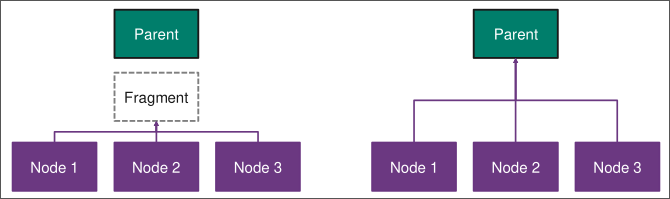
\includegraphics[width=\columnwidth]{2022-10-18-11_31_01.png}

\subsection{EventListener}  
An event listener is used to bind a function to something like a button\newline
For example a darkmode button is mapped to the useDarkMode function
\vspace{-2mm}
\begin{lstlisting}
document.querySelector('button')
.addEventListener('click' // action to map , useDarkMode // function to map,[options] // once, capture etc)
\end{lstlisting}
\vspace{2mm}


\subsection{remove Eventlistener and dispatchEvent}  
You can of course also remove an eventlistener, or execute an event per js call:
\vspace{-2mm}
\begin{lstlisting}
document.querySelector('button').removeEventListener('click', useDarkMode);
// remove eventlistener

document.querySelector('button').dispatchEvent('click');
// dispatch the click event
\end{lstlisting}
\vspace{2mm}

\subsection{NodeStructure}  
\textcolor{orange}{HTML is built like a tree with different nodes and leafs.}\newline
\textcolor{teal}{Important is that there are different types of nodes that html uses}
\begin{itemize}
  \item \textcolor{orange}{ElementNode} head,body,li,title etc
  \item \textcolor{orange}{AttributeNode} href, charset, src etc
  \item \textcolor{orange}{TextNode} some text to display
  \item \textcolor{orange}{Comments} <!-- kekw -->
\end{itemize}
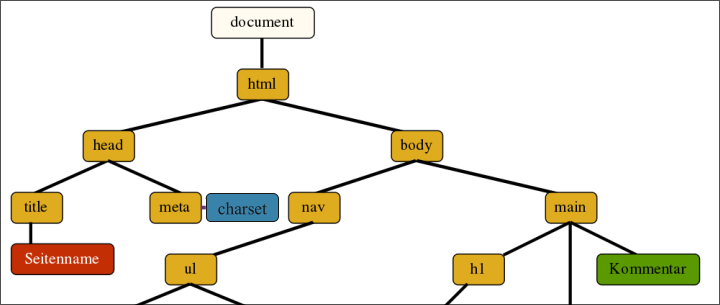
\includegraphics[width=\columnwidth]{2022-10-18-10_35_52.png}

\subsection{async and defer}  
\textcolor{orange}{\textbf{async:}}\newline
Async means that the script will be loaded and executed immediately.\newline
This means that there \textbf{is no guarantee for order} and the script will be \textbf{executed before the document has loaded}.\newline
\textcolor{blue}{\textbf{defer:}}\newline
This is the opposite to async, it will \textbf{gurarantee order}, \newline
and the document will \textbf{be loaded before the script executes}.
\minipg{
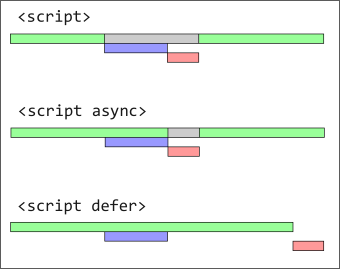
\includegraphics[width=\columnwidth]{2022-10-18-10_45_27.png} 
}{
Events:
\begin{itemize}
\item \textcolor{orange}{DOMContentLoaded}\newline
  Document parsed, but images etc are loading
\item \textcolor{orange}{load}\newline
  both are ready
\end{itemize} 
Legend:
\begin{itemize}
\item \textcolor{green}{HTML Parsing}
\item \textcolor{gray}{HTML parsing paused}
\item \textcolor{blue}{Script Download}
\item \textcolor{red}{Script Execution}
\end{itemize}
}[0.15,0.1]
\textcolor{orange}{\textbf{If you want to check whether or not the document is ready, \newline
then you can do this with: }}\textcolor{red}{\textbf{\emph{document.readyState}}}


\subsection{TextContent and innerText}  
\textcolor{orange}{HTMLElement.innerText provides the rendered text with css applied}\newline
\textcolor{blue}{HTMLElement.textContent provides the complete raw text with no css applied}
 
\subsection{className and classList}  
\vspace{-2mm}
\begin{lstlisting}
<script>
console.log(
document.querySelector("#el").className);
// box alert important

console.log(document.querySelector("#el")
.classList);
// DOMTokenList(3) ["box", "alert", "important"]
</script>
\end{lstlisting}
\vspace{2mm}


\subsection{Event Handling}

\subsubsection{EventListener with options}  
\vspace{-2mm}
\begin{lstlisting}
target.addEventListener(type, listener[, options]);
\end{lstlisting}
\vspace{2mm}
options:
\begin{itemize}
  \item capture \newline
    Whether or not the element in question should catch the event during capture phase
  \item once \newline
    Whether or not the eventhandler should function \textbf{only once}
  \item passive \newline
    Specifies that the function in question \textbf{will not call PreventDefault()}
  \item signal \newline 
    Specifies that the eventlistener will be removed if the \textbf{AbortSignals associated abort() method is called}
  
\end{itemize}

\subsubsection{Event Listener vs inline}  
\vspace{-2mm}
\begin{lstlisting}
// dynamic eventype: multiple listeners possible!
document.querySelector("#1").addEventListener("click", () => alert('1'));

// fixed type: only 1 listener possible
// will overwrite previous onclick assignments
document.querySelector("#2").onclick = () => alert('2');

// inline: provides the least amount of flexibility, not recommended
<button onclick="alert('3')">3</button>
\end{lstlisting}
\vspace{2mm}

\subsubsection{Event Phases} 
\textcolor{orange}{Events go through 3 phases:}\newline
\begin{enumerate}
  \item \textcolor{teal}{Capture-Phase}\newline
    Event travels from root to leaf\newline
    Every Element can react here
  \item \textcolor{teal}{Target-Phase}\newline
    Event will be executed on target
  \item \textcolor{teal}{Bubble-Phase}\newline/
    Event travels from leaf to root\newline
    Each element can react
\end{enumerate}
\vspace{2mm}
\textcolor{orange}{Event bubbling and capture is used to dynamically change lists, etc.}\newline
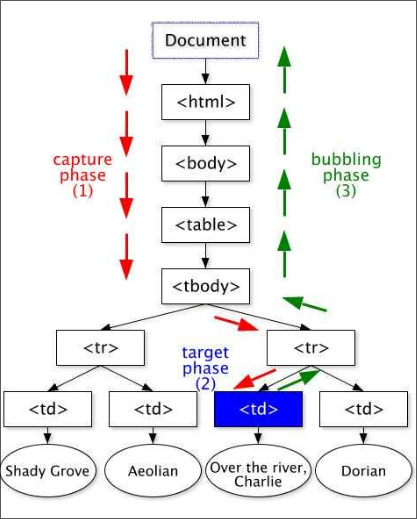
\includegraphics[width=0.7\columnwidth]{2022-10-18-12_15_49.png}

\subsection{Node}

\subsubsection{Important Properties and functions} 
\minipg{
\textcolor{orange}{\textbf{Properties}}
\begin{itemize}
  \item \textcolor{teal}{children} only nodes of type HTMLelement 
  \item \textcolor{teal}{childNodes} 
  \item \textcolor{teal}{firstChild} first node child
  \item \textcolor{teal}{firstElementChild} first element child
  \item \textcolor{teal}{nextSibling} next node sibling
  \item \textcolor{teal}{nextElementSibling} next element 
  \item \textcolor{teal}{parentElement} 
\end{itemize}
}{
\textcolor{orange}{Functions}
\begin{itemize}
  \item \textcolor{teal}{appendChild()}
  \item \textcolor{teal}{removeChild()}
  \vspace{2mm}
  \vspace{2mm}
  \vspace{2mm}
  \vspace{2mm}
  \vspace{2mm}
\end{itemize}
}[0.17,0.09]

\subsection{Element}

\subsubsection{Important Properties and functions}
\minipg{
\textcolor{orange}{\textbf{Properties}}
\begin{itemize}
  \item \textcolor{teal}{id} 
  \item \textcolor{teal}{className} 
  \item \textcolor{teal}{classList} 
  \item \textcolor{teal}{innerHTMl}
\end{itemize}
}{
\textcolor{orange}{Functions}
\begin{itemize}
  \item \textcolor{teal}{getAttribute()}
  \item \textcolor{teal}{setAttribute()}
  \item \textcolor{teal}{toggleAttribute()}
  \item \textcolor{teal}{closest()}
\end{itemize}
}[0.1,0.1]

\subsubsection{Element ParentNode}  
\textcolor{orange}{Element also implements Parentnode:}\newline
\minipg{
\textcolor{orange}{Properties:}
\begin{itemize}
  \item \textcolor{teal}{children}
  \item \textcolor{teal}{firstElementChild}
  \item \textcolor{teal}{lastElementChild}
\end{itemize}
}{
\textcolor{orange}{Functions:}
\begin{itemize}
  \item \textcolor{teal}{append()} 
  \item \textcolor{teal}{remove()}
\end{itemize}
}[0.1,0.1]

\subsection{HTMLElement}

\subsubsection{Important Properties and functions}  
\minipg{
\textcolor{orange}{\textbf{Properties}}
\begin{itemize}
  \item \textcolor{teal}{dataset} 
  \item \textcolor{teal}{style} 
  \item \textcolor{teal}{hidden}
\end{itemize}
}{
\textcolor{orange}{Functions}
\begin{itemize}
  \item \textcolor{teal}{createCaption()}
  \item \textcolor{teal}{createTFoot()}
  \item \textcolor{teal}{createTHead()}
\end{itemize}
}[0.1,0.1]

\subsection{Event-Object}

\subsubsection{Important Properties and functions}  
\textcolor{orange}{\textbf{Properties}}
\begin{itemize}
  \item \textcolor{teal}{target} // element of event origin 
  \item \textcolor{teal}{currentTarget} // element that has listener for this event
\end{itemize}
\textcolor{orange}{Functions}
\begin{itemize}
  \item \textcolor{teal}{preventDefault()} // prevents default actions like automatic form submit
  \item \textcolor{teal}{stopPropagation()} // stops capturing and bubbling
\end{itemize}
\textcolor{orange}{Specific Event types}
\begin{itemize}
  \item \textcolor{teal}{MouseEvent}
  \item \textcolor{teal}{WheelEvent}
  \item \textcolor{teal}{InputEvent}
  \item \textcolor{teal}{KeyboardEvent}
\end{itemize}

\subsection{Keyboard Event}  
\minipg{
\begin{itemize}
  \item change: what changed?
  \item keydown: which key has been pressed?
  \item ctrlKey: was the control pressed during keydown?
\end{itemize}
}{
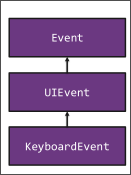
\includegraphics[width=\columnwidth]{2022-10-18-12_33_39.png}
}[0.17,0.07]
\vspace{-2mm}
\begin{lstlisting}
document.querySelector("input").addEventListener("keydown", (event) => {
  console.log(event.key);
})
\end{lstlisting}
\vspace{2mm}

\section{Scopes}

\subsection{Var vs let}  
Usually we declare variables using the let keyword, however, the old var keyword still has one technicality that the let keyword doesn't have. Namely the var keyword will always be available for the parent scope:
\vspace{-2mm}
\begin{lstlisting}
{ // empty explicit scope to show difference
  function some_func() {
    let num1 = 5;
    var num2 = 6;
    console.log(num1); // ok -> 5
    console.log(num2); // ok -> 6
  }
    console.log(num1); // -> undefined!
    console.log(num1); // ok -> 6
}
\end{lstlisting}
\vspace{2mm}

\subsection{Scope per file in NodeJs} 
NodeJs creates an additional scope per file, this means that you essentially can only explicitly declare a truly global variable with var.\newline
\textcolor{red}{However, the browser does \textbf{NOT} have this feature!}

\subsection{Closure}  
This is just the concept of boxing a something in something and then accessing the scope from the inner "something". Usually done with functions:
\vspace{-2mm}
\begin{lstlisting}
function something1() {
  let num = 5;
  function something2() {
    console.log(num); // obviously works
  }
}
\end{lstlisting}
\vspace{2mm}

\subsection{global Scope}  
If you access a global variable, it is probably better to use the \textbf{global.variable} naming scheme. The reason for this is obviously the fact that you don't use the variable of another scope by accident.

\subsection{This in scopes}  
if we do not have an object, then the \textbf{the global scope will be this!}\newline
This means that you can do things like this:
\vspace{-2mm}
\begin{lstlisting}
function printName() {
  console.log(this.name);
}
const name = "ping"

const logEntry = {
  name: "pang"
};
logEntry.printName = printName;
logEntry.printName(); // will print "pang"
printName(); // will print "ping" -> empty object will always invoke the global object!!
\end{lstlisting}
\vspace{2mm}

\subsection{Functions with new (old js)}  
\textcolor{orange}{Before proper OOP was introduced, this was the way you wrote OOP in js:}\newline
\vspace{-2mm}
\begin{lstlisting}
// given the code from above, we create another printName instance with new
// this will create an empty object that will be the "instance" to call the method on
new printName();

// This is what happens under the hood when you call new printName()!
// function newPrintName() {
//   var self = {}
//   console.log(self.name);
//   return self;
// }
\end{lstlisting}
\vspace{2mm}

\subsection{This as a parameter}  
\textcolor{orange}{You can also pass the this keyword as a parameter!}\newline
\vspace{-2mm}
\begin{lstlisting}
logEntry.printName({name: "pingpang"});
// this will print "pingpang" instead of the logEntry name "pang" !!
\end{lstlisting}
\vspace{2mm}

\subsection{Bind}  
You can also "bind" a certain "this" to one function in particular, this means that all other function other than the one you bound, will be used with the regular "this"!!\newline
\vspace{-2mm}
\begin{lstlisting}
const bindPrintName = logEntry.printName({ name: "burrmiu" });
bindPrintName(); // this will ALWAYS print "burrmiu"
// at least until you override it!
bindPrintName({name: "pangPing!"}); // !!!! this will still print "burrmiu" !!!!
\end{lstlisting}
\vspace{2mm}


\section{Strict Mode in JS}


\subsection{Basic} 
This disables certain JS features that might be unwanted in this particular usecase. \newline
It can be enabled per Scope or per file\newline
\textcolor{purple}{Usually this simply makes JS throw an exception when you would expect it from other functions,for example when using a method with a "this" but used on nothing -> exception instead of using global scope.}

\subsection{Usage}  
\vspace{-2mm}
\begin{lstlisting}
function someFunc() {
  'use strict'; // this enables the strict mode for this particular scope or file
  // for compatability, should a browser use old js without this feature, then the strict will simply be ignored
}
\end{lstlisting}
\vspace{2mm}

\subsection{General}  
All new features in JS are in strict mode, this essentially forces us to use it, and it is generally good practice to simply use the strict mode!

\section{Lambda}

\subsection{Notation}  
\vspace{-2mm}
\begin{lstlisting}
let x = (parameter) => {
  // Do something
  console.log(parameter);
};
x(5); // will print 5!
\end{lstlisting}
\vspace{2mm}

\subsection{This in Lambda} 
In Lambdas the this is always based on the parent scope.\newline
For example within a function or a class the this will be based on that function or class:
\vspace{-2mm}
\begin{lstlisting}
function Point(x, y){
  this.x = x;
  this.y = y;
  this.area = () => this.x + this.y;
}
var areaFn = new Point(10,50).area;
console.log(areaFn());

// explicit version!
// function Point(x, y) {
//   var _this = this; // here the _this is mapped to this!
//   this.x = x;
//   this.y = y;
//   this.area = function () {
//     return _this.x + _this.y;
//   };
// }
\end{lstlisting}
\vspace{2mm}


\section{Objects and Classes}

\subsection{Objects are Hashtables!} 
Every object is a hashtable, this means that we have different means to access it's values. \newline
The same thing therefore applies to arrays as well as long as there is a name for it:
\vspace{-2mm}
\begin{lstlisting}
const items = {name: "pingpang"};

console.log(items.name);
console.log(items["name"]);
// these are both the same!
\end{lstlisting}
\vspace{2mm}
\textcolor{purple}{Since js does not have static types, you can also add something like name: "ping" to an array and access it the same way you access any other object, however this is \textbf{not recommended!}}

\subsection{Classes} 

\begin{itemize}
\item \textcolor{purple}{\#: This is the prefix for private variables}
\item \textcolor{purple}{super: Superclass call}
\item \textcolor{purple}{instanceof: this checks whether or not,\newline
  an instance is an object of class xyz\newline
Note, subclasses are also instanceof parentclass!}
\end{itemize}
\vspace{-2mm}
\begin{lstlisting}
class Clock {
  #timer // the # makes it private!
  currentTime
  constructor(param) {
    super();
  }
  start() {
    this.#timer = setTimeout(() => { 
      this.currentTime = new Date();
    }, 1000);
  }
  get time() {
    return this.currentTime
  }
  set time(newTime) {
    this.currentTime = newTime
  }
}
const clock = new Clock(); // instance
\end{lstlisting}
\vspace{2mm}

\subsection{Classes before JS6}  
The prototype keyword was used to use OOP before JS6, this is still used under the hood, but do not use this anymore unless you have performance issues.

This Context with Lambda Callbacks 
\textcolor{red}{This code below does not work, the reason for this is that when we pass person.wackUP, we lose the this context, as we only pass the function itself!}\newline
\vspace{-2mm}
\begin{lstlisting}
class Person {
  constructor(name) {
    this.name = name;
  }
  wackUp() {
    console.log(`${this.name} is awake!`)
  }
}
class Alarm {
  registerAlarm(callback) {
    setTimeout(() => {
      callback()
    }, 1000);
  }
}
const person = new Person("Michael");
const alarm = new Alarm();
alarm.registerAlarm(person.wackUp);
\end{lstlisting}
\vspace{2mm}
\textcolor{red}{In order to preserve the context, we can pass the function as a lambda:}\newline
\vspace{-2mm}
\begin{lstlisting}
alarm.registerAlarm(() => person.wackUP() );
\end{lstlisting}
\vspace{2mm} 
\textcolor{red}{The same can be done in the class itself!!}\newline
\vspace{-2mm}
\begin{lstlisting}
wackUp = () => {
  console.log(`${this.name} is awake!`)
}
\end{lstlisting}
\vspace{2mm}

\section{Modules}

\subsection{UseCase}  
The use case is as expected the prevention of namespace issues.\newline
For example every script in the browser is in the global scope, this means that if the index.js and the home.js both have a function called hello(), then they will overwrite each others definition!!\newline
\textcolor{purple}{The other usecase is \textbf{dependency solving} and \textbf{code departmentalization}.}\newline
\textcolor{teal}{In Node.js the file need to end with .mjs in order to use modules, in the browser the ending .js is fine.}\newline
\textcolor{teal}{Modules are \textbf{ALWAYS STRICT!}}

\subsection{Definition}  
\textcolor{purple}{\textbf{Modules simply export or import values and functionality to or from other modules!}}

\subsection{Module Usage}  
\textcolor{red}{\textbf{In order to use a module, the file itself needs to be a module!}}\newline
\vspace{-2mm}
\begin{lstlisting}
<script src="index.js" type="module"></script>
\end{lstlisting}
\vspace{2mm}
\textcolor{orange}{The usage is done with the import keyword:}\newline
\vspace{-2mm}
\begin{lstlisting}
import {register as alarmClock} from './libs/alarm-clock.js'
import {register as newsFeed} from './libs/news-feed.js'
import * from './pingpang.js' // import every export from this file 
import defaultExport from './something.js' // default export explained below
\end{lstlisting}
\vspace{2mm}

\subsection{Export}
\textcolor{purple}{There are 2 types of exports, \textbf{named} and \textbf{unnamed}.}\newline
\vspace{2mm}
\textcolor{orange}{\textbf{Named Export}: In order to export a function or value, you need to use the export keyword before that function/value:}\newline
\vspace{-2mm}
\begin{lstlisting}
export someFunc() {
  console.log("pingpang");
}
\end{lstlisting}
\vspace{2mm}
\textcolor{orange}{\textbf{defaultExport}: Here we define an export at the end of the file:}\newline
\vspace{-2mm}
\begin{lstlisting}
export default {name: "pangping"};

// in the import file
console.log(defaultExport.name);
\end{lstlisting}
\vspace{2mm}



\section{Advanced JS Features}

\subsection{Set Timeout}
\vspace{-2mm}
\begin{lstlisting}
const timer = setTimeout(() => {
  // perform this after x amount of miliseconds
}, 1000); // 1000 miliseconds!
clearTimeout(timer); // kills the timer -> call before timer ends
\end{lstlisting}
\vspace{2mm}

\subsection{Spread}  
\textcolor{orange}{Spread is a feature that allows fast and easy concatenation of arrays just like in haskell:}
\vspace{-2mm}
\begin{lstlisting}
const listA = [1,2,3,4,5];
const listB = [10,11,12,13,14];
const listC = [...listA, ...listB];

// this can also be done with other objects

const objA = {name: "ping"};
const objB = {name2: "pang"}; // can't have same key twice!
const objC = {...objA,...objB}; // this copies the values of objA and objB into objC
const objD = {objA,objB}; // this however copies the full object into it

console.log(objC); // {name: "ping", name2: "pang"}
console.log(objD); // {objA: {name: "ping"}, objB: {name2: "pang"}}
// note the extra curly braces on the objD -> deep copy!
\end{lstlisting}
\vspace{2mm}

\subsection{Spread Operator as parameter}  
\textcolor{orange}{You can also enter an array as a parameter:}
\vspace{-2mm}
\begin{lstlisting}
function something(a,b,c) {
  return a + b + c;
}
const arr = [1,2,3,4,5,6,7,8,9];
something(...arr); // this works -> a=1,b=2,c=3, rest ignored
\end{lstlisting}
\vspace{2mm}

\subsection{Destructuring}  
\textcolor{orange}{You can create variables directly from an array or object:}
\vspace{-2mm}
\begin{lstlisting}
const [a, b] = [10,20]; // a = 10, b = 20 
const {c, d} = {name: "pang", price: 50};

function something({message}) {
  console.log(message);
}
something({message:"pangping"}) // prints "pangping"!

function printWithDefaults({message = "message"} = {}) { // object destructuring
console.log(message);
}
printWithDefaults({code: "error_1"}) // error_1
printWithDefaults() // message
\end{lstlisting}
\vspace{2mm}

\subsection{Nullish Operator}  
In case you want to check if for example a number exists, even a 0, you can use the nullish operator.\newline
This will simply use the value in case it exists, or the default value that you have specified if it is undefined or null.
\vspace{-2mm}
\begin{lstlisting}
console.log(0 ?? 42); // will print 0 
console.log(undefined ?? 42); // will print 42
\end{lstlisting}
\vspace{2mm}


\subsection{Optional chaining}  
In JS you might always encounter values that are undefined, this often leads to issues where you call a function with undefined values, or even worse the entire function is undefined.\newline
We can counteract this with the Optional Operator:
\vspace{-2mm}
\begin{lstlisting}
const item = {
  name: "pangping",
  price: 10, 
  fun: {
    word: "no"
  }
};
console.log(item.fun?.word); // this will print "no" IF the fun object exists!
// otherwise we simply do not execute this code, no exception will be thrown.
\end{lstlisting}
\vspace{2mm}


\section{Clean Code}

\subsection{Naming}  
\textcolor{orange}{Names of variables, function etc should be \textbf{short, intuitive and explicit}.}\newline
\textcolor{teal}{Also the names should be \textbf{spellable} and consisting of \textbf{kown words}, something that you can't say is useless in coop programming.}\newline
\textcolor{purple}{Avoid repeating yourself, if the app is about webtrc, you don't need to specify this every time!}

\subsection{Naming schemes}  
\textcolor{orange}{There are different schemes for different types of variables that you use.}
\begin{itemize}
\item \textcolor{purple}{regular variables and functions >> camelCase}
\item \textcolor{purple}{constants >> ALL\_CAPS}
\item \textcolor{purple}{boolean values >> isValue}
\item \textcolor{purple}{arrays >> pluralNaming}
\end{itemize} 

\subsection{Functions}  
Function should also be \textbf{short, fitting name for functionality, pos-x compliant} -> only 1 functionality and \textbf{as few parameters as possible}
\textcolor{purple}{Naming:}\newline
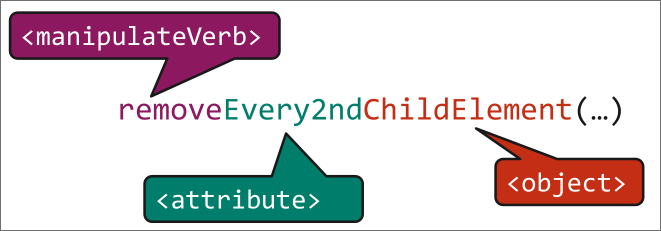
\includegraphics[width=0.6\columnwidth]{2023_02_02_04_51_04.png}

\subsection{Code Smells}  
Names
\begin{itemize}
\item \textcolor{purple}{useless Names}
\item \textcolor{purple}{too short names}
\item \textcolor{purple}{too abstract names}
\end{itemize}
Functions
\begin{itemize}
\item \textcolor{purple}{too many parameters}
\item \textcolor{purple}{too much dead code -> not reached code}
\item \textcolor{purple}{Function too long}
\item \textcolor{purple}{boolean flags}
\end{itemize} 
Comments
\begin{itemize}
\item \textcolor{purple}{outdated comments}
\item \textcolor{purple}{superfluous comments}
\item \textcolor{purple}{commented code}
\end{itemize} 
More
\begin{itemize}
\item \textcolor{purple}{Code duplicates}
\item \textcolor{purple}{Inconsistent formatting}
\item \textcolor{purple}{Inconsistent naming across functions and names}
\end{itemize}


\section{PolyFill and BabelJS}

\subsection{BabelJS}  
BabelJS converts new and modern JS code into old style JS, this is used for compatibility with older browsers that do not support the new features.

\subsection{PolyFill} 
BabelJS has certain limitations that PolyFill tries to essentially "fill in". This further increases the compatibility with older browsers, however, this still is limited to a certain extend.\newline
For example due to the translating, the performance will be much worse, and considering we are already using an older browser, this can quickly get out of hand.

\subsection{Model View Controller (MVC)}  
This is essentially an abstract system to create web-applications, it abstracts 3 different things: the \textbf{view -> Display of data}, the \textbf{model -> app state}, and the \textbf{Controller -> reaction to input}\newline
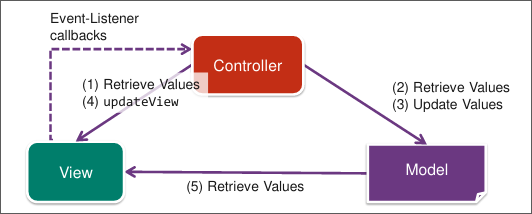
\includegraphics[width=\columnwidth]{2022-11-08-11_39_15.png}\newline
\textcolor{teal}{You can create this for every project that you would create with the tri-force html/css/js}

\subsection{Example for MVC}  
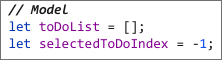
\includegraphics[width=0.5\columnwidth]{2022-11-08-11_42_52.png}\newline
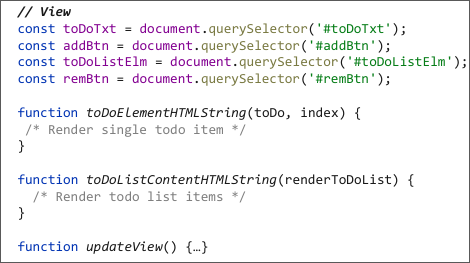
\includegraphics[width=0.8\columnwidth]{2022-11-08-11_42_58.png}
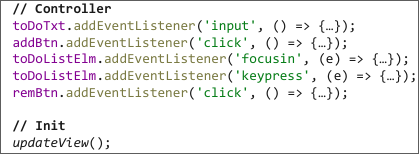
\includegraphics[width=0.8\columnwidth]{2022-11-08-11_43_08.png}


\section{npm}

\subsection{Basics Commands}  
\begin{itemize}
\item \textcolor{purple}{npm init} -> create a new project
\item \textcolor{purple}{npm install} -> install all packages needed for this project
\item \textcolor{purple}{npm run} -> run the project
\end{itemize} 

\subsection{Packages in npm}  
Each node package has its own \textbf{package.json}.\newline
This specifies \textbf{the name, the type, the version, main file, description and dependencies}:\newline
Here an example package:\newline
\vspace{-2mm}
\begin{lstlisting}
{
  "name": "my-package",
  "type": "module",
  "version": "1.0.0",
  "main": "index.js",
  "description": "My first node package",
  "dependencies": {
    "ws": "^7.3.1"
  }
  "devDependencies": {
    "stylelint": "^13.13.1"
  }
}
\end{lstlisting}
\vspace{2mm}

\section{AJAX Asynchronous JavaScript and XML}

\subsection{Creating a small Server}  
\vspace{-2mm}
\begin{lstlisting}
// imports and config
import http from 'http';
const hostname = '127.0.0.1'
const port = 3000

// handler for requests
const server = http.createServer((req, res) => {
  res.statusCode = 200
  res.setHeader('Content-Type', 'text/plain')
  res.end('Hello World\n')
})

// start the server
server.listen(port, hostname, () => {
  console.log(
  `Server running at http://${hostname}:${port}/`)
})
\end{lstlisting}
\vspace{2mm}

\subsection{Use Case}  
The problem with js is that it is singlethreaded, this means that only one thing can be done at a time.\newline
This makes things like animations problematic, as they can be blocked by requests, clicks etc.\newline
To solve this the async engine handles a "queue", which means that a request might \textbf{not be executed immediately, but whenever there is a "free space for it"}\newline
Other Effects that AJAX made possible:
\begin{itemize}
\item \textcolor{purple}{Single Page Applications}
\item \textcolor{purple}{Animations and other changes without refreshing}
\item \textcolor{purple}{Data via "best effort", UI via "guaranteed"}
\end{itemize} 

\subsection{Promise}  
This states that \textbf{at some point you will receive an answer}, however, \textbf{there is no guarantee for the value}, it can be anything or even null/undefined.\newline
\textcolor{OliveGreen}{A promise has 3 states, \textbf{Fulfilled, Pending and Rejected}, fulfilled means the action was successfull and a return value is available, pending means operation still active and rejected means the action has failed}
\vspace{-2mm}
\begin{lstlisting}
async function fetchFromURL() {
  return new Promise ((resolve, reject) => {
  const response = fetch('https://stone.sifs0005.infs.ch/ranking')
    .then(res => res.json())
    .then(json => resolve(json))
  }).catch(
    err => reject(err)
  );
}
\end{lstlisting}
\vspace{2mm}

\subsection{Constructor of Promise}  
\vspace{-2mm}
\begin{lstlisting}
new Promise((resolve, reject) =>
// call async func with arguments
>>>async fn<<< (..., (...callbackArgs) => {
  if (error) {
    reject(error);
  } else {
    resolve(value);
  }
})
\end{lstlisting}
\vspace{2mm}
As you can see a promise has 2 functions as parameters that will handle the 2 possible end states reject -> rejected and resolve -> fulfilled.

\subsection{Using promises}  
You can either use promises with the \textbf{.then()} function, or with the \textbf{await} keyword.
\vspace{-2mm}
\begin{lstlisting}
// with .then()
function fetchFromURLThen() {
  feetch('https://dashie.org/something').then(
    (response) => {
      console.log(response);
    }
  );
}
// with await
async function fetchFromURLAwait() { //async needed!!
  const response = await fetch('https://dashie.org/something');
  console.log(response); // note response is just a code!
} // use .json, .text etc to get the data!!
\end{lstlisting}
\vspace{2mm}
\textcolor{red}{Note: with await you need to classify the function as async!!}\newline
Error handling with promises:\newline 
\vspace{-2mm}
\begin{lstlisting}
async function getGreeting(fetchURL) {
  try { 
    return await fetch(fetchURL); 
  } catch (e) {
    console.error(e);
  }
}
// or with .then
async function getGreeting(fetchURL) {
  .then((response) => {
    return response; 
  }).catch((e) => {
    console.log(e);
  })
}
\end{lstlisting}
\vspace{2mm}
\textcolor{purple}{Manual promise usage:}
\vspace{-2mm}
\begin{lstlisting}
const p1 = Promise.reject('no'); // rejects with error 'no'
const p1 = Promise.resolve(42);  // creates promise
p1.then(x => console.log(x))); // unpacks promise and logs 42
\end{lstlisting}
\vspace{2mm}

\section{REST Representational State Transfer}
\textcolor{purple}{Services that implement this are called "RESTful"}\newline
This is a style of transerring resources without side effects, this means that \textbf{we only transer data, there will be no function calls!}.
\begin{itemize}
\item \textcolor{purple}{Client-Server based}
\item \textcolor{purple}{Stateless communication}
\item \textcolor{purple}{Cacheable}
\item \textcolor{purple}{Layered System} Load balancers, proxies and firewalls
\item \textcolor{purple}{Unified Interface}
\end{itemize} 

\subsection{Richardsons Maturity Model}  
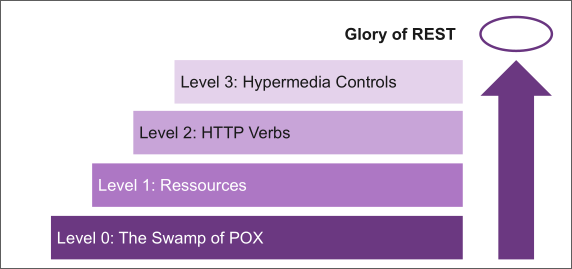
\includegraphics[width=0.8\columnwidth]{2022-11-29-11_08_34.png}

\subsection{Level 0: The Swamp of POX}  
Here we \textbf{send each request individually}, we send plain \textbf{xml} messages.\newline
Each request is sent to the \textbf{same endpoint}. 
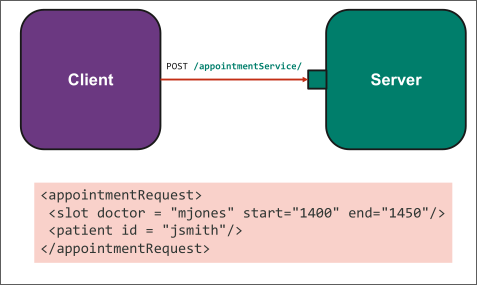
\includegraphics[width=0.8\columnwidth]{2022-11-29-11_14_31.png}


\subsection{Level 1: Resources}  
With this level we can receive data from different endpoints, this essentially allows \textbf{divide and conquer} -> "multithreading".\newline 
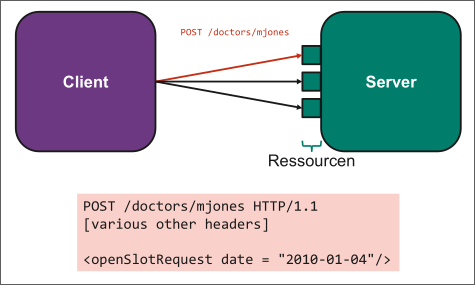
\includegraphics[width=0.7\columnwidth]{2022-11-29-11_14_57.png}

\subsection{Level 2 HTTP-Verbs}  
Now we can use different html methods like \textbf{GET or POST}, this distinguishes the idea of pushing or getting data, making it easier to handle data apropriately. \newline
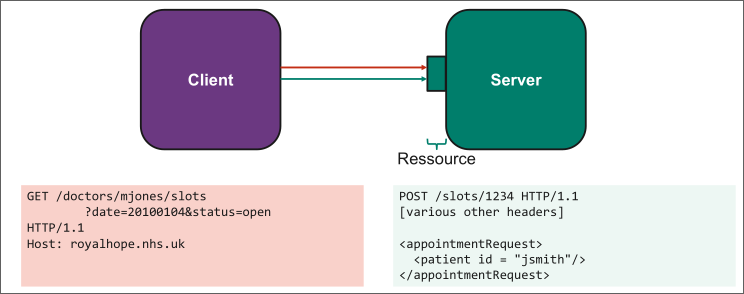
\includegraphics[width=0.9\columnwidth]{2022-11-29-11_17_08.png}

\subsection{Level 3: Hypermedia Controls}  
We now can include \textbf{states of the application}, this allows us to specify the exact usecase even further, making it easier to handle the data accordingly:\newline
Level 3 also gives us the ability to \textbf{specify possible actions} with this data, eg. book an appointment via an \textbf{URI}.
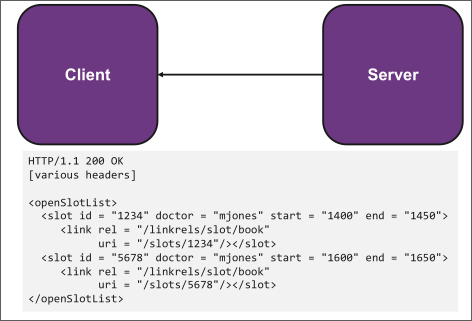
\includegraphics[width=0.7\columnwidth]{2022-11-29-11_19_32.png} \newline
\textcolor{red}{Note the link rel and uri, which specify possible actions to take!}

\subsection{REST vs RPC (Remote Procedure Call)}  
REST is much simpler, this allows a much cleaner implementation of function on your side, and also gives you much more flexibility as to what and how you implement things. \newline
The downside is that at some point RPC will be easier when you get to a certain dependency on each other, in other words, loosely connected applications benefit from the REST concept, while strongly connected ones benefit from RPC.\newline 
\textcolor{orange}{In general REST is better for data requests, as it is based on resources instead of calls}

\subsection{Resource Oriented Architectures (ROA)}  

\begin{itemize}
\item \textcolor{purple}{Resource}\newline
  Everything that is important enough to get its own id
\item \textcolor{purple}{Name}\newline
  unique ID of a resource
\item \textcolor{purple}{Representation}\newline
  Can be done in multiple ways, html, xml, whatever
\item \textcolor{purple}{Links}\newline
  Hyperlinks connect resources
\item \textcolor{purple}{Interface}\newline
  Uniform Interface\newline
  Standard HTML methods
\item \textcolor{purple}{Stateless Communication}
\end{itemize} 

\subsection{HTTPS Request}  
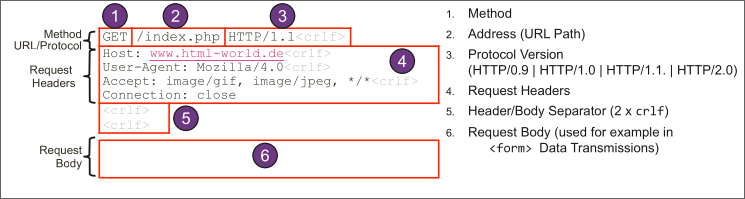
\includegraphics[width=\columnwidth]{2022-11-29-11_35_27.png}

\subsection{HTTPS Response}
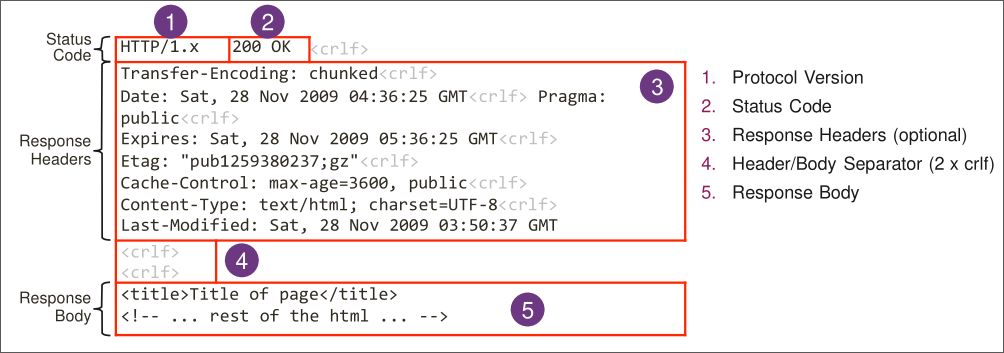
\includegraphics[width=\columnwidth]{2023_02_02_04_59_15.png}

\subsection{Response Codes}
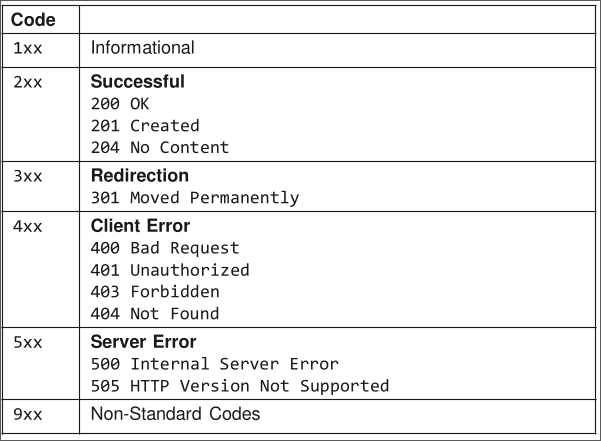
\includegraphics[width=0.7\columnwidth]{2023_02_02_05_00_11.png}

\subsection{Example Requests in JS}
\vspace{-2mm}
\begin{lstlisting}
async function getJson(url) {
  const response = await fetch(url);
  return response.json();
} // GET Request
async function postJson(url, json) {
  const response = await fetch(url, {
    method: 'post',
    headers: {
      'Accept': 'application/json',
      'Content-Type': 'application/json',
    },
    body: JSON.stringify(json),
  });
  return response.json();
} // Post Request
\end{lstlisting}
\vspace{2mm}

\subsection{OpenAPI Documentation and JSON Server}
\vspace{-2mm}
\begin{lstlisting}
{ // JSON server
"posts": [{
"id": 1,
"title": "json-server",
"author": "xxx"
}, {
"title": "WED1 is great",
"author": "markus",
"id": 2
}],
// OpenAPI
paths:
  /board:
  get:
      summary: Get the whole board description: Retrieves the current state
               of the board and the winner.
      parameters: ...
      responses:
          "200":
              description: Everything went fine.
              content: ...
  put: ...
\end{lstlisting}
\vspace{2mm}

\subsection{Query filter, sort}  
\vspace{-2mm}
\begin{lstlisting}
// filter
orders?state=activeseller_id=1234
// sort
orders?order-by=date&order-direction=asc
// Pagination
GET /companies?skip=10&take=10
\end{lstlisting}
\vspace{2mm}

\subsection{Important HTTP Methods}  
\minipg{
\begin{itemize}
\item \textcolor{purple}{GET}\newline
  Request resources
\item \textcolor{purple}{POST}\newline
  Create resources
\item \textcolor{purple}{PUT}\newline
  Update or Create resources
\end{itemize} 
}{
  \begin{itemize}
\item \textcolor{purple}{DELETE}\newline
  Delete resources
\item \textcolor{purple}{PATCH}\newline
  Partial updates
  \, \newline
  \, \newline
  \end{itemize} 
}[0.15,0.1]

\subsection{Best practices}  
\begin{itemize}
\item \textcolor{black}{Use JSON as it is native to JS}
\item \textcolor{black}{Use correct HTML methods}
\item \textcolor{black}{Use html status codes}
\item \textcolor{black}{API is only as good as its documentation}
\item \textcolor{black}{Limit data sent and received}
\end{itemize} 

\subsection{Nielsen}  
This is a system of things to comply with:\newline
\begin{itemize}
\item \textcolor{purple}{Visibility of System State}\newline
  For example, display the steps that a program does when the user waits, instead of a generic message saying "please wait for shit to finish"
\item \textcolor{purple}{Connection between real world and system}
\item \textcolor{purple}{Freedom and Control for the user}
\item \textcolor{purple}{Consistency and Standards}
\item \textcolor{purple}{Avoiding Errors}
\item \textcolor{purple}{Remember states instead of asking about them}
\item \textcolor{purple}{Flexibility and efficient Usage}
\item \textcolor{purple}{Asthetics and minimalistic Design}
\item \textcolor{purple}{Support of Detection and Resolution of Problems}
\item \textcolor{purple}{Support and Documentation}
\end{itemize} 

\subsection{Suspense State} 
Inform the user when your system needs to load something and is currently doing so. Also consider removing/disabling UI elements that wouldn't work during this time, e.g. sending the request again!
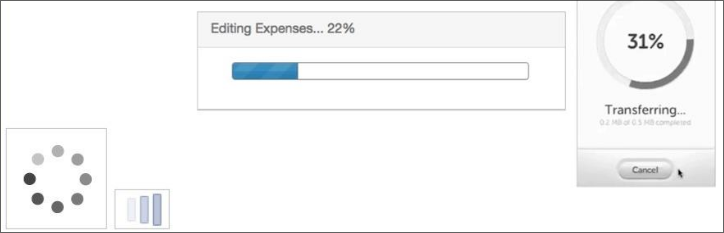
\includegraphics[width=0.8\columnwidth]{2022-12-06-11_30_22.png}

\subsection{Debouncing and Preempting}
When trying to create a Search Machine, you want to show the possible completions, however this costs a GET request with each letter.\newline
Instead we wait a few miliseconds to see if the user will write another character and only then send the request. -> \textcolor{purple}{\emph{Debouncing}}\newline
In case we already want a new request before the last has been processed, \textcolor{purple}{\emph{we cancel it preemptively -> preempting}} and send the new one.\newline 
\textcolor{purple}{Throttling:} simply reduce the amount of requests....

\subsection{Polling and Sockets}
When trying to receive Information from a server, you can either \emph{poll the server in specific timeframes (high load on server)}, or you can agree on a \emph{mutual timeframe where the server send you data -> socket}.

\section{Usability}

\subsection{Peripheral vs Central Vision}  
The idea is that changes outside of the central vision are hard to notice, meaning that it is often not recommended to show errors and changes outside of that vision, however, sometimes too much things popping up in the central vision can be irritating when doing some work, see "fabio rages yet again at steams fucking popup for an update"\newline

\subsection{UI element Intuitiveness / Affordance}  
In general UI elements should work as expected, text fields should take inputs, buttons should be clickable, radio buttons should only allow one selection, etc.\newline
\textcolor{purple}{The easiest way to guarantee this is to make a connection to the real world, does it work the way everything else does?}

\subsection{Consistency}  
Do not make sudden changes with your design language or your UI elements, it should be consistent all across your website, buttons should always work the same way, radio buttons should always work the same way, etc.

\subsection{Rules of design}  
\begin{itemize}
\item \textcolor{purple}{Rule of Similarity}\newline
  \begin{itemize}
  \item \textcolor{black}{Similar things need to close together}
  \item \textcolor{black}{Based on colors, sizes, shapes, movements}
  \item \textcolor{black}{Generate contrasts to other elements}
  \item \textcolor{black}{Take level of similarity into account -> amount of similarities}
  \end{itemize} 
\item \textcolor{purple}{Rule of Distance}\newline
  \begin{itemize}
  \item \textcolor{black}{Things that are close together will be considered a group by the human eye}
  \item \textcolor{black}{Therefore neighbours should always be in a group}
  \item \textcolor{black}{Make clear distinctions from one group to the other}
  \end{itemize} 
\item \textcolor{purple}{Rule of Conciceness}\newline
  You should not provide unnecessary information and UI elements -> material design
\item \textcolor{purple}{Rule of Simplicity}\newline
  Less is often more, again -> Material Design
\item \textcolor{purple}{Rule of equal direction}\newline
  Items that are grouped should be facing the same direction
\item \textcolor{purple}{Rule of Closed system}\newline
Your design should be considered a closed system, meaning that it does not use the entirety of the screen
\end{itemize}
\vspace{2mm}

\includegraphics[width=0.8\columnwidth]{2022-12-13-11_37_23.png}

\subsection{Colors}  
\begin{itemize}
\item \textcolor{purple}{Use less than 6 colors}
\item \textcolor{purple}{Use colors in the general application}\newline
  green for go, red for stop
\item \textcolor{purple}{Make sure contrasts make sense}
\item \textcolor{purple}{use color schemes}
\end{itemize} 

\subsection{Usability Tests}  
These are done in order to check if the target audience can/does use the product in question as intended.\newline
\textcolor{orange}{Often designers have a use case in mind, but users might not directly understand how it is meant to be used, and therefore misuses it.}\newline
In other words, see if the old boomer dude can use the app as well if they are part of the indented audience, or if only a bunch of nerds can use it -> TUI.


\lstdefinelanguage{CSS}{
    sensitive=true,
    keywords={%
    % JavaScript
    typeof, new, true, false, catch, function, return, null, catch, switch, var, if, in, while, do, else, case, break,
    % HTML
    html, title, meta, style, head, body, script, canvas,
    % CSS
    color:, border-radius:, border:, transform:, -moz-transform:, transition-duration:, transition-property:,
    transition-timing-function, background:, background-size:, background-color:, background-image:, background-origin:, background-repeat:, background-position:, background-attachement:, border:, border-box:, border-width:, border-color:, border-bottom:, border-style:, border-radius:, border-spacing:, border-collapse:, text-transform:, text-decoration-thickness:, text-align:, text-indent:, text-shadow:, text-justify:, text-overflow:, text-decoration:, text-align-last:, text-decoration-line:, text-decoration-color:, text-decoration-style:, margin:, padding:, 
    },
    % http://texblog.org/tag/otherkeywords/
    otherkeywords={<, >},   
    ndkeywords={class, export, boolean, throw, implements, import, this},   
    comment=[s]{/*}{*/},
    morecomment=[l]//,
    morecomment=[s]{<!}{>},
    morestring=[b]',
    morestring=[b]",    
    alsoletter={-},
    alsodigit={:}
}
\lstset{
    language=CSS,
    style=code,
}
%%%%%

\section{CSS}
\subsection{Syntax and Selectors}
\vspace{-2mm}
\begin{lstlisting}
body { /* thing to change the style of */ 
    color: red; /* style changes */
}
\end{lstlisting}
\vspace{2mm}
\textcolor{purple}{Selectors}
\begin{itemize}
\item \textcolor{orange}{\#hello} id
\item \textcolor{orange}{.something} class -> here class something
\item \textcolor{orange}{div} element -> here element div
\item \textcolor{orange}{p::before} pseudo-element, here selects non-existing element before p
\item \textcolor{orange}{p:hover} pseudo-class, selected when you hover over p element
\item \textcolor{orange}{a[ href]} attribute select: selected when href is set in a element
\end{itemize} 
\, \newline
\textcolor{purple}{Comments:}
\vspace{-2mm}
\begin{lstlisting}
/* This is a comment*/ 
/* This is a 
multiline comment */
\end{lstlisting}
\vspace{2mm}
\, \newline
\textcolor{purple}{Colors}
\vspace{-2mm}
\begin{lstlisting}
color: red; /* or */ color: #55667788; /* #RRGGBBAA */
\end{lstlisting}
\vspace{2mm}

\subsubsection{Stylesheets vs Inline}
\textcolor{purple}{Inline css, and <style> (DO NOT USE!)}
\vspace{-2mm}
\begin{lstlisting}
<p style="color:red;"> /* inline css */
    This is a paragraph.
</p>
<style> /* full css inside html */
body {
  background-color: linen;
}
</style>
\end{lstlisting}
\vspace{2mm}

\textcolor{purple}{Proper Stylesheets}
\vspace{-2mm}
\begin{lstlisting}
<link rel="stylesheet" href="style.css">
<link rel="stylesheet" href="https://dashie.org"> 
/* css style is in that file, note: second is online! */ 
\end{lstlisting}
\vspace{2mm}

\subsubsection{Inherit and initial}
\vspace{-2mm}
\begin{lstlisting}
color: value|initial|inherit;
/* initial = default value, inherit = parent value*/
\end{lstlisting}
\vspace{2mm}
\textcolor{purple}{Specificity of inherit and initial are 0!}\newline
\textcolor{orange}{If you want something to use inheritance then you need to explicitly state this!}

\subsubsection{Base Specificity}
\begin{enumerate}
\item \textcolor{orange}{Browser defaults}
\item \textcolor{orange}{Webpage defined by dev}
\item \textcolor{orange}{Browser settings by user}
\end{enumerate} 

\subsubsection{Specificity on page}
\textcolor{orange}{This applies to the part that is defined by the developer!}\newline
\textcolor{purple}{There are 4 counters:} (theoretically 6) -> user and important
\begin{itemize}
\item \textcolor{orange}{a:} Inline styles
\item \textcolor{orange}{b:} ID selectors
\item \textcolor{orange}{c:} Class, pseudo class and attribute selectors
\item \textcolor{orange}{d:} element and pseudo-element selectors
\end{itemize}
\minipg{
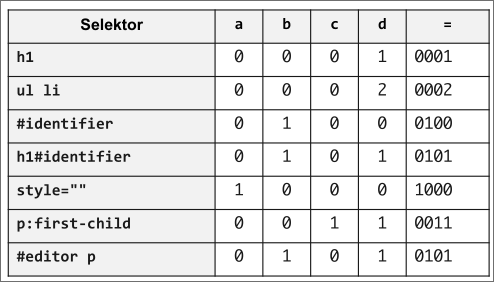
\includegraphics[width=\columnwidth]{2023_02_02_03_52_26.png}
}{
  \begin{itemize}
  \item \textcolor{black}{The * has specificity 0}\newline
    \textcolor{purple}{the * stands for \emph{everything}}
  \item \textcolor{black}{The :not() is ignored, but not the contents inside of it}
  \end{itemize} 
}[0.15,0.09]
\textcolor{purple}{Cascade:}\newline
The css style will be applied starting with the lowest value selector, therefore the higher values will override the lower ones!

\textcolor{purple}{Override with !important:}
\vspace{-2mm}
\begin{lstlisting}
h1 {
font-weight: bold;
font-size: 20px; !important; /* specificity: 120001 */
} /* due to important this is the MOST specific! */
#h1 {
font-size: 30px; /* specificity: 021000 */
} /* ignored because important tag -> font-size is 20 */
\end{lstlisting}
\vspace{2mm}
\textcolor{red}{Should always be avoided if you can!}

\subsubsection{Specific Selection}
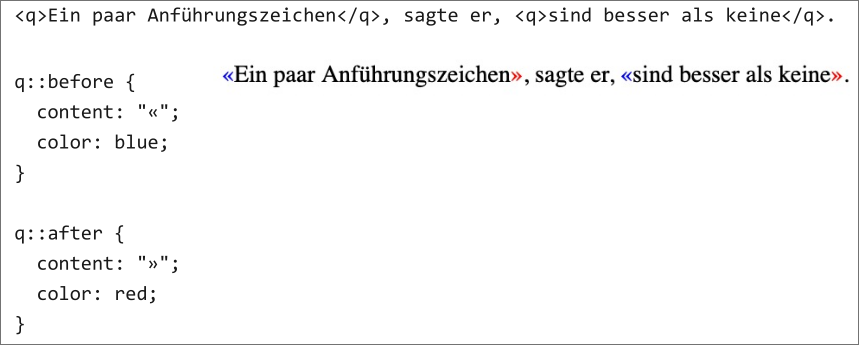
\includegraphics[width=0.9\columnwidth]{2022-10-04-10_58_46.png}
\textbf{Combinators and selectors}  
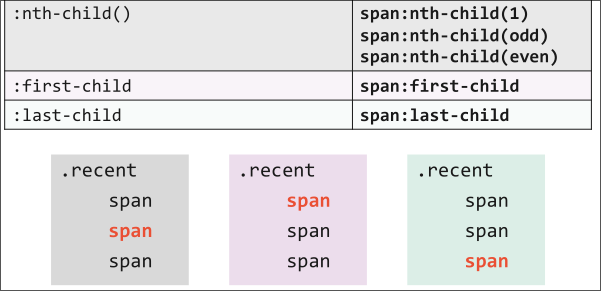
\includegraphics[width=0.8\columnwidth]{2022-10-04-11_03_12.png}\newline 
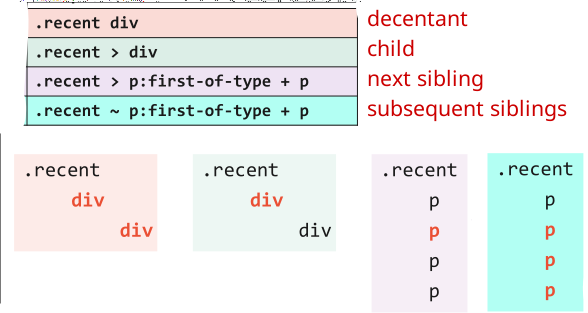
\includegraphics[width=0.7\columnwidth]{2022-10-04-11_03_26.png}\newline
\textcolor{purple}{:is pseudo class selector}
\vspace{-2mm}
\begin{lstlisting}
:is (box, button, something) p:hover {
background-color: red;
something-else: value;
} /* less writing than box p:hover, buttom p:hover ... */
\end{lstlisting}
\vspace{2mm}
\textcolor{purple}{:has pseudo class selector}
\vspace{-2mm}
\begin{lstlisting}
div:has(p.error) {
  border: 1px solid red;
} /* selects divs that have p.error as child */
\end{lstlisting}
\vspace{2mm}
\vspace{-2mm}
\begin{lstlisting}
tr.warning td:nth-child(1)::before{
  color: red;
  content: "\26A0";
}
\end{lstlisting}
\vspace{2mm}
 This selects the td of a tr in class warning. Then goes to the nth-child, here 1 and before the content of said td.\newline
Then you can add new content with content: "something";\newline
Keep in mind that any changes with color etc are only made to this new content, as you specify it above!\newline

\textcolor{purple}{Hiding an element:}
\vspace{-2mm}
\begin{lstlisting}
some-element::before {
  display: none;
} /* element is only hidden, not deleted! */
\end{lstlisting}
\vspace{2mm}

 \subsection{Pseudo selectors in JS}  
\textbf{You can't use the CSS pseudo selectors in JS without some weird hacks, therefore, JS has some specific elements inbuilt like first-child, last-child and more.}

\subsection{Units}
\minipg{
\textcolor{purple}{Relative size}
\begin{itemize}
\item \textcolor{orange}{em:} relative to parent font-size
\item \textcolor{orange}{rem:} relative to the root font-size
\item \textcolor{orange}{ch:} relative to the character"0"
\item \textcolor{orange}{vh:} relative to viewport height
\item \textcolor{orange}{vw:} relative to viewport width
\item \textcolor{orange}{\%:} relative to parent size
\end{itemize} 
}{
  \textcolor{purple}{Fixed size}
\begin{itemize}
\item \textcolor{orange}{px}
\item \textcolor{orange}{mm}
\item \textcolor{orange}{cm}
\item \textcolor{orange}{in}
\, \newline
\, \newline
\, \newline
\end{itemize} 
}[0.15,0.1]

\subsection{Background}
\vspace{-2mm}
\begin{lstlisting}
background-color: red;
background-image: "/path"; /* can also be an url -> url(https://...)*/
background-size: cover|auto|length|percentage|contain;
// cover: resizes to parent, auto: size of image, contain: resize image to fit inside parent, initial: fixed x,y value
background-position: x-value y-value; // top right, top center, center center, ...   Can also be x% y% default 0% 0%.
background-attachement: scroll|fixed|local; // local: scrolls with element, scroll is default.
// this decides if the background scrolls with the page or not.
background-origin: padding-box|content-box|border-box; 
// Used to define where the background image starts inside a box, only works when background-attachement is not fixed.
background-repeat: repeat|repeat-x|repeat-y|no-repeat|space|round; //useless shit
\end{lstlisting}
\vspace{2mm}

\subsection{Borders}
\vspace{-2mm}
\begin{lstlisting}
border: 4px solid red;
border: border-width border-style border-color;
border-style: none|hidden|dotted|dashed|solid|double|groove|ridge|inset|outset|initial|inherit;
//styles like ridge, groove, inset and outset use 3D effects, hard to describe.
border-radius: 4px 4px 4px 4px; // border-radius: 5px; also possible
//borders can be addressed individually by specifying a direction:
border-bottom: 4px solid red;
border-collapse: separate|collapse|initial|inherit;
// collapse means borders will merge in boxes. seperate will draw borders for both elements.
border-spacing: 4px; //Spacing between borders if the border-collapse is enabled!
\end{lstlisting}
\vspace{2mm}


\subsection{Margins and Paddings}
\vspace{-2mm}
\begin{lstlisting}
margin: top right bottom left;
margin: 10px 10px 10px 10px; /* == margin: 10px; */
padding: top right bottom left;
padding: 10px 10px 10px 10px;
//margin-right padding-left etc work as well.
\end{lstlisting}
\vspace{2mm}
Margin is the spacing between the element itself and it's parent and or other elements in the same hierarchy.\newline
Padding is the spacing inside the element to the contents of said element.

\subsection{Text}
\vspace{-2mm}
\begin{lstlisting}
text-align: left|right|center|justify; // justify is text as a block.
text-align-last: left|right|center|justify; //The last line can be configured indiidually.
text-justify: auto|inter-word|inter-character|none; /* only used when text-align is set to justify.
inter-word increases spacing between words, inter-character for characters.*/
text-decoration: text-decoration-line text-decoration-color text-decoration-style text-decoration-thickness;
text-decoration-line: none|underline|overline|line-through;
text-decoration-style: solid|double|dotted|dashed|wavy;
text-decoration-thickness: auto|from-font|value;
text-indent: value;
text-overflow: clip|ellipsis|string; 
//clip will just cut the string off, ellipsis ends with ..., a string will display itself.
text-shadow: h-shadow v-shadow blur-radius color|none;
text-transform: none|capitalize|uppercase|lowercase;
\end{lstlisting}
\vspace{2mm}

\subsubsection{Fonts}
\vspace{-2mm}
\begin{lstlisting}
font: font-style font-variant font-weight font-size/line-height font-family
|caption|icon|menu|message-box|small-caption|status-bar; //use the font used by this element
font-style: normal|italic|oblique; //oblique seems to be the same as italic.
font-variant: normal|small-caps;
font-weight: normal|bold|bolder|lighter|number; //number in 100 steps -> 100,200,300,...,900
font-size: medium|xx-small|x-small|small|large|x-large|xx-large|smaller|larger|length;
line-height: normal|number|length;
font-family: family-name|generic-family; //generic-family example: Isoveka
\end{lstlisting}
\vspace{2mm}

\subsection{Boxes}
\subsubsection{Display, justify and align}
\vspace{-2mm}
\begin{lstlisting}
display: none|flex|grid|inline|block|contents|inline-block|inline-flex|inline-grid|inline-table|list-item|run-in|table|table-caption|table-column-group|table-footer-group|table-row-group|table-cell|table-column|table-row;
\end{lstlisting}
\vspace{2mm}
\textcolor{purple}{Center Div or other HORIZONTALLY}\newline 
You can center a box horizontally by using the \textbf{display: flex or display: grid} on the parent box, as well as \textbf{justify-content: center} on the parent box\newline
\textcolor{purple}{Center Div or other VERTICALLY}\newline 
You can center a box vertically by using the \textbf{display: table} on the \emph{parent of the parent} and using \textbf{display: table-cell} on the parent.\newline 
\textcolor{red}{Important note for CSS: Position is usually relative and based on parent attributes, this means that centering etc must usually be done in the parent!}

\subsubsection{Information about flexbox}
dynamically allocates spaces for elements inside this element.
usually combined with justify-content to adjust element position.\newline 
\textcolor{purple}{min-height and min-width}\newline 
Use this instead of fixed height or width, as it allows your page to scale with bigger screens!


\subsubsection{Types of Boxes}
\textbf{\emph{content-box and border box}}
  \textbf{content-box} increases the box size to ensure the child \textbf{element has the set size}.\newline
  \textbf{border-box} decreases the element size to ensure \textbf{the box itself has the set size}.
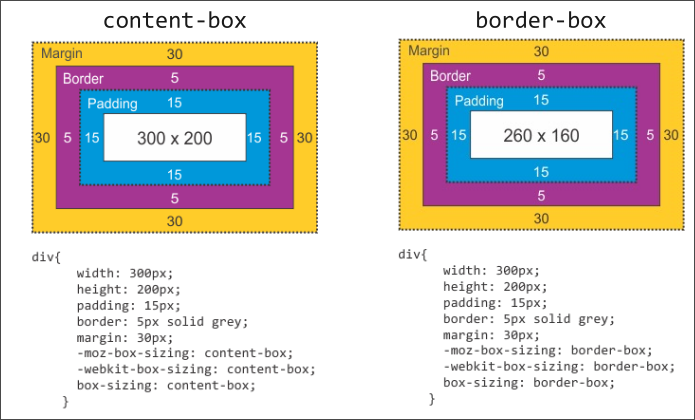
\includegraphics[width=\columnwidth]{2022-10-04-11_35_35.png}




\lstdefinelanguage{HTML}{
    sensitive=true,
    keywords={%
    % JavaScript
    typeof, new, true, false, catch, function, return, null, catch, switch, var, if, in, while, do, else, case, break,
    % HTML
    html, title, meta, style, head, body, script, canvas,
    % CSS
    color:, border-radius:, border:, transform:, -moz-transform:, transition-duration:, transition-property:,
    transition-timing-function, background:, background-size:, background-color:, background-image:, background-origin:, background-repeat:, background-position:, background-attachement:, border:, border-box:, border-width:, border-color:, border-bottom:, border-style:, border-radius:, border-spacing:, border-collapse:, text-transform:, text-decoration-thickness:, text-align:, text-indent:, text-shadow:, text-justify:, text-overflow:, text-decoration:, text-align-last:, text-decoration-line:, text-decoration-color:, text-decoration-style:, margin:, padding:, 
    },
    % http://texblog.org/tag/otherkeywords/
    ndkeywords={class, export, boolean, throw, implements, import, this},   
    comment=[s]{/*}{*/},
    morecomment=[l]//,
    morecomment=[s]{<!--}{-->},
    morestring=[b]',
    morestring=[b]",    
    alsoletter={-},
    %otherkeywords={<, >},   
    alsodigit={:}
}
\lstset{
    language=HTML,
    style=code,
}
%%%%%


\section{HTML Hypertext Markup Language}

\textbf{\emph{HTML is not a programming language}}, it is a markup language.\newline
HTML simply defines \textbf{content} and \textbf{structure}.

\subsection{Example HTML File}
\vspace{-2mm}
\begin{lstlisting}
<!DOCTYPE html>
<html lang="en">
<head> <!-- Metadata only, not displayed! -->
  <meta charset="UTF-8">
  <link rel="stylesheet" href="styles/global.css">
  <link rel="shortcut icon" href="#">
  <title>Rock Paper Scissors</title>
</head> <!-- not the same as header! -->
<body>
  <!-- other stuff -->
  <script src="scripts/main.js" type="module"></script>
</body>
\end{lstlisting}
\vspace{2mm}

\subsection{Basic Syntax and Information}
\textcolor{purple}{Comments:}
\vspace{-2mm}
\begin{lstlisting}
<!--This is an html comment!-->
<!--This is a 
multiline comment!-->
\end{lstlisting}
\vspace{2mm}

\textcolor{purple}{Tags}
\vspace{-2mm}
\begin{lstlisting}
<input type="text" placeholder"enter something">
<!-- optional /> inside the tag above (discouraged) -->
<!-- no </input>! (empty tag!) -->
\end{lstlisting}
\vspace{2mm}
Certain elements like <title> are only allowed in the header, others like <h> are only allowed in the body.\newline
You can technically just use these tags without specifying the body and header.\newline
However this might be confusing to some people.
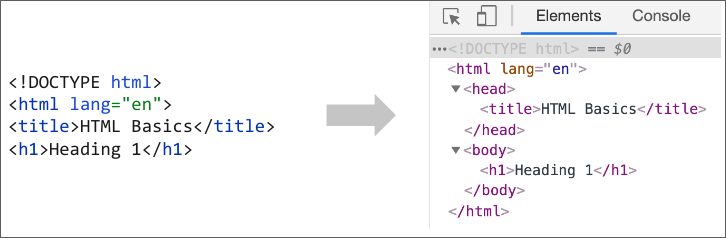
\includegraphics[width=0.8\columnwidth]{2022-09-27-10_53_50.png}


\subsubsection{Semantic Markup}
-- HTML offers a variety of tags specifically made for a usecase, these also work well with screenreaders etc\newline
-- It also helps with recognition in search engines.\newline
-- Mobile support is also likely to be better with proper html.

\subsubsection{Semantic Element, what to choose?}
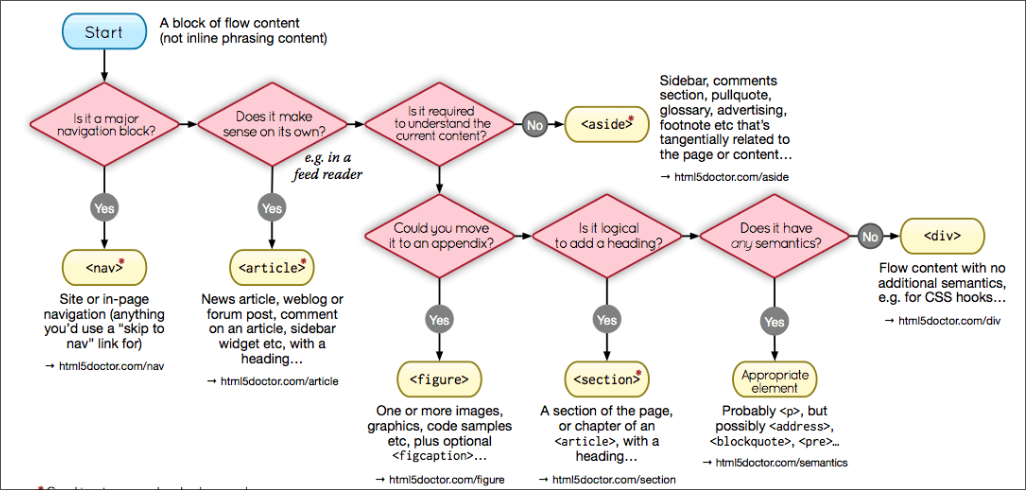
\includegraphics[width=\columnwidth]{2022-09-27-11_45_58.png}

\subsubsection{Base Elements}
\textcolor{purple}{Categories of Elements}
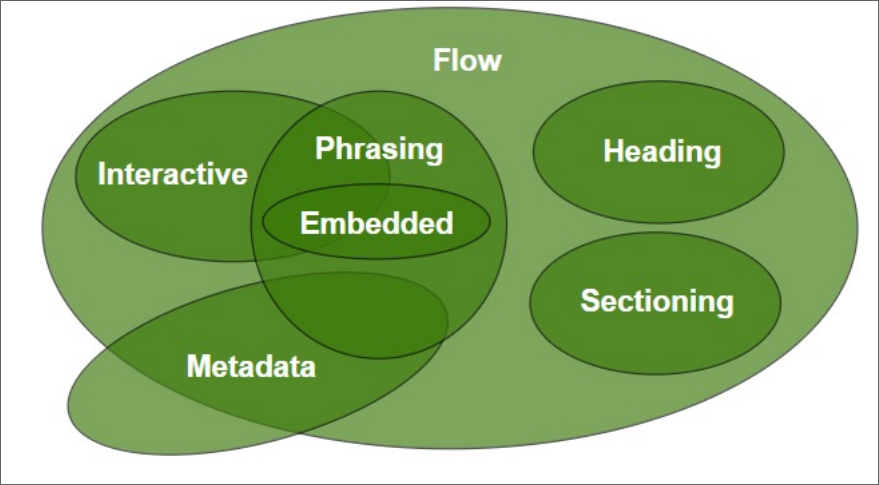
\includegraphics[width=0.8\columnwidth]{2023_02_02_01_44_10.png}

\textcolor{purple}{Image <img> (empty tag, embedded/interactive)}
\vspace{-2mm}
\begin{lstlisting}
<img src="path to source" alt="alternative text">
\end{lstlisting}
\vspace{2mm}

\textcolor{purple}{Input <input> (empty tag, interactive)}
\vspace{-2mm}
\begin{lstlisting}
<input type="text" placeholder="something">
\end{lstlisting}
\vspace{2mm}

\textcolor{purple}{Form with js function <form> (interactive)}
\vspace{-2mm}
\begin{lstlisting}
<form onsubmit={() => handleSubmit()}><!-- elements --></form>
\end{lstlisting}
\vspace{2mm}

\textcolor{purple}{Header-text, from 1 to 6 <h1> (heading)}
\vspace{-2mm}
\begin{lstlisting}
<h1>Some text to use as header</h1> <!--h1,h2,h3,h4,h5,h6-->
\end{lstlisting}
\vspace{2mm}

\textcolor{purple}{Paragraph <p> (phrasing)}
\vspace{-2mm}
\begin{lstlisting}
<p>Some text to display</p>
\end{lstlisting}
\vspace{2mm}

\textcolor{purple}{Ordered List <ol> / <ul> (flow)}
\vspace{-2mm}
\begin{lstlisting}
<ol>
    <li>element1</li>
    <li>element2</li>
</ol>
\end{lstlisting}
\vspace{2mm}

\textcolor{purple}{Hyperlink <a> (interactive)}
\vspace{-2mm}
\begin{lstlisting}
<a href="htts://dashie.org">Shitgaem</a>
\end{lstlisting}
\vspace{2mm}

\textcolor{purple}{bold text <b> (phrasing)}
\vspace{-2mm}
\begin{lstlisting}
<b>this text is bold, or maybe not.</b>
\end{lstlisting}
\vspace{2mm}

\textcolor{purple}{italic text <em> (phrasing)}
\vspace{-2mm}
\begin{lstlisting}
<em>This text is italic, or maybe not</em>
\end{lstlisting}
\vspace{2mm}

\textcolor{purple}{div <div> (flow)}
\vspace{-2mm}
\begin{lstlisting}
<div>try centering it!</div>
\end{lstlisting}
\vspace{2mm}

\textcolor{purple}{Navigation Bar <nav> (sectioning)}
\vspace{-2mm}
\begin{lstlisting}
 <nav>
  <a href="/html/">HTML</a> |
  <a href="/css/">CSS</a> |
  <a href="/js/">JavaScript</a> |
</nav>
\end{lstlisting}
\vspace{2mm}

\textcolor{purple}{Bar on the side <aside> (sectioning)}
\vspace{-2mm}
\begin{lstlisting}
<aside>Something to display on the side</aside>
\end{lstlisting}
\vspace{2mm}

\textcolor{purple}{article <article> (sectioning)}
\vspace{-2mm}
\begin{lstlisting}
<article><!-- other elements --></article>
\end{lstlisting}
\vspace{2mm}

\textcolor{purple}{section <section> (sectioning)}
\vspace{-2mm}
\begin{lstlisting}
<section><!-- this should always have a heading! --></section>
<!-- The difference to article is that section is not independent! it always has a heading. -->
\end{lstlisting}
\vspace{2mm}

\subsubsection{Global Attributes}
Basic attributes, self-explanatory
\begin{itemize}
\item \textcolor{purple}{id, hidden, title, lang, class, accesskey, draggable, hidden}
\item \textcolor{purple}{onclick, oncancel, contentedible, spellcheck, title (extra information)}
\end{itemize} 

\textcolor{purple}{Special Attributes}
\begin{itemize}
\item \textcolor{orange}{dir:} specifies the direction of text
\item \textcolor{orange}{style:} specifies inline css, don't use!
\item \textcolor{orange}{tabindex:} tabbing order of an element
\item \textcolor{orange}{Aria Attributes:} Accessible Rich Internet Applications\newline
  This is used to re-purpose elements with proper accessibility, only use if nothing else works!
\end{itemize} 
\, \newline

\textcolor{purple}{Custom Attributes with data-*:}\newline
You can name an attribute data-eventtype and use it as follows:
\vspace{-2mm}
\begin{lstlisting}
document.querySelector("pingpang").addEventListener("click", (event) => { 
  if (event.target.getAttribute("data-eventtype") == "add") {
   rerender();
  } else {
    console.log("pingpang!");
  }
})
\end{lstlisting}
\vspace{2mm}
\textbf{This makes sure you don't use the same function for every single bubbling event!}\newline
\, \newline

\textbf{\textcolor{red}{Tag Omission}}\newline 
Certain tags can be omitted in special cases:\newline
<html>, <body>, <head>, <p>, <li>.\newline
When exactly they can be omitted is found on the MDN\newline
\textcolor{purple}{It is not recommended to omit tags!}

\section{JS exceptions}
\vspace{-2mm}
\begin{lstlisting}
"4" / "2"               //=> 2: Number
"4" - "2"               //=> 2: Number
"4" * "2"               //=> 8: Number
"4" + "2"               //=> '42': String
10 * 3 + "px"           //=> '30px': String
8 * "1px"               //=> NaN: Number
"px" + 1 -2             //=> NaN: Number
"3px" + 3 * 2 + "3px"   //=> '3px63px': String
"foo" ++ "abc"          //=> 'fooNaN': String
"2" - -1                //=> 3 :Number
[] + []                 //=> '': String
[] + {}                 //=> '[object Object]' :String
{} + []                 //=> 0: Number
{} + {}                 //=> '[object Object][object Object]'
[] == false             //=> true
[] === false            //=> false
[] == 0                 //=> true
[] == "0"               //=> false -> unexpected!
[] == ![]               //=> true
[] === ![]              //=> false
0 == "0"                //=> true
0 === "0"               //=> false
"" == false             //=> true
"" === false            //=> false
null == undefined       //=> true
null === undefined      //=> false
[1,2] == "1,2"          //=> true
[1,2] === "1,2"         //=> false
NaN == NaN              //=> false
NaN === NaN             //=> false
(1-"i") == (1-"i")      //=> false: (NaN == NaN)
false === false         //=> true
4 === 4                 //=> true
false === true          //=> false
true + true + true == 3 //=> true 
true - true             //=> 0   
true == 1               //=> true
true === 1              //=> false
a={0,1,2}               //=> true
a[3] === undefined      //=> true
a[3] == null            //=> false
a[3] === null           //=> 4   
parseInt("4k", 10)      //=> NaN 
parseInt("4k", 2)       //=> 140: = 4*30^1 + k*30^0
parseInt("4k", 30)      //=> NaN
Number("4k")            //=> 4
Number("4")              
\end{lstlisting}

\end{multicols*}
\end{document}

